
\documentclass{IOS-Book-Article}
\usepackage[utf8]{inputenc}
\usepackage{graphics}
\usepackage{graphicx}
\usepackage{mathptmx}
\usepackage{soul}\setuldepth{article}
\usepackage{hhline,longtable}
\usepackage{float}
\usepackage{placeins}
\usepackage{multicol}
\usepackage[english]{babel}
\usepackage{bbding, wasysym, fontawesome, amssymb}
\let\Cross\relax
\usepackage{marvosym}

\graphicspath{{figures/}}
%\usepackage{hhline, colortbl, longtable}
%\usepackage{times}
%\normalfont
%\usepackage[T1]{fontenc}
%\usepackage[mtplusscr,mtbold]{mathtime}
%
\def\hb{\hbox to 10.7 cm{}}

\begin{document}

\pagestyle{headings}
\def\thepage{}


\begin{frontmatter}              % The preamble begins here.


%\pretitle{Pretitle}
\title{IoT-Based Smart Medicine Dispenser to Control and Supervise Medication Intake\\}

\markboth{}{}
%\subtitle{Subtitle}

\author[A]{\fnms{Gleiston} \snm{GUERRERO-ULLOA}%
\thanks{Corresponding Author: Gleiston Guerrero-Ulloa, Faculty of Engineering Sciences, Quevedo State Technical University, 120501 Quevedo, Ecuador. E-mail: gguerrero@uteq.edu.ec}},
\author[B]{\fnms{Miguel J.} \snm{Hornos}}
,
\author[B]{\fnms{Carlos} \snm{Rodríguez-Domínguez}}
and
\author[A]{\fnms{Ma. Mercedes} \snm{FERNÁNDEZ-COELLO}}

\runningauthor{G. Guerrero-Ulloa et al.}
\address[A]{Faculty of Engineering Sciences, Quevedo State Technical University, Ecuador}
\address[B]{Software Engineering Department, University of Granada, Spain}

\begin{abstract}. This paper presents a system consisting of a smart medicine dispenser of solid medications (pills, capsules,…) and a mobile application for its configuration and management. The main idea is to offer a solution to help people (especially vulnerable ones) to avoid incorrect medication intakes. In this regard, the smart dispenser delivers the required medication if two conditions are met: (1) it is the scheduled time for a medication intake, and (2) the person who removes the medication from the dispenser (patient or caregiver) can be identified and is authorized to do so. Person identification and authorization is performed through facial recognition by the dispenser and through a username and a password by the mobile application. Moreover, the system reminds the users whenever a medication intake should take place through mobile notifications and lights and sounds emitted by the dispenser. The system development has been guided by a Test-Driven Development Methodology for Internet of Things (IoT)-based Systems to promote its quality and reliability.
	
\end{abstract}

\begin{keyword}
Smart system\sep medicine dispenser\sep facial recognition\sep mobile application\sep Internet of Things (IoT)\sep elderly


\end{keyword}
\end{frontmatter}
\markboth{}{}
%\thispagestyle{empty}
%\pagestyle{empty}

\section{Introduction}

Population ageing is a worldwide concern, due to the system-changing effects that it implies: well-being and social policies, economical sustainability, availability of public services, etc. For example, according to the United Nations \cite{r1}, 36.81\% of the forecasted population (16,062,075 people) will be elderly (over 65 years old) in Spain by 2050. Likewise, 22.35\% of the United States of America population (84,813,265 people) will also be elderly by that year.

Nonetheless, life expectancy is steadily growing every year. According to the data published by the European Commission, life expectancy in Europe in 2018 was between 70.1 (Latvia) and 81.9 years old (Switzerland), and has an average growth of 0.3 years per year \cite{r2}. That is, it could be roughly in the range between 80 and 92 years old by 2050.

One of the side effects of the population ageing is the widespread impact of many chronic diseases and conditions: diabetes, high blood pressure, heart conditions, cognitive impairment, etc. In that sense, researchers are proposing Internet of Things (IoT)-based systems and smart environments to help elderly people to deal with their consequences \cite{r3,r5}. One of the aids that these systems can offer is to remind and ease medication intakes.

Chronic diseases usually require people to intake many different medications at a very steady schedule. However, due to cognitive decline, elderly people are more prone to intake medications in a wrong way (e.g., more or less intakes than expected, at a different schedule, mix-up medications, etc.) \cite{r6}. In fact, according to Singh et al. \cite{r7}, an estimated 25\% of the elderly population does not intake their medication according to the professional prescription. A wrong medication intake can lead to many negative situations, such as health worsening, increased amount of hospitalizations, or even a premature death \cite{r8,r9,r10}.

In this paper, we present a system consisting of a smart medicine dispenser and a mobile application for its configuration and management. The dispenser emits a sound and lights up an LED to alert the patient that it is time to take his/her medication. When he/she is close to the smart medicine dispenser, it will identify him/her through facial recognition and deliver the prescribed medication. If the medication is not removed during the expected timings, a notification is sent to the caregiver through the mobile application so that she/he can act consequently. The mobile application can also deliver reminders to those patients able to use a smartphone. This is useful when they are not close to the dispenser at the schedule time for a medication intake. Moreover, it allows registering several patients, as well as managing the medication schedule and even multiple smart dispensers.
 
The remainder of this paper is structured as follows. Section 2 presents some previous works related to smart medicine dispensers. Section 3 describes the proposed system. Finally, Section 4 outlines our conclusions and future work.

\section{Related Works}

IoT is a lifestyle transforming computing paradigm \cite{r11} that can even lead to the fourth industrial revolution \cite{r12,r13}. Furthermore, IoT is an opportunity for many researchers to propose smart systems to help people in many domains, among them those that emit reminders to people to assist them during their daily life at home.
For instance, an IoT-based system prototype to offer light, sound and voice reminders to elderly people through a chair is proposed in \cite{r6}. Another work with the same goal is presented in \cite{r14}, but using a photo frame to emit a set of reminders that are previously configured through a mobile application. In both cases, reminders are generic, that is, they do not have a specific goal.

Many other systems are specifically designed to deliver medication-related reminders. However, in a comparison of some existing medicine dispensers \cite{r8}, the conclusion was that most of the existing proposals do not rely on an Internet connection (i.e., they do not allow remote operation) and do not have any user interaction.

Nonetheless, more recent related works do use Internet. For example, a smart medicine flask that delivers reminders according a pre-established schedule is presented in \cite{r15}, while a medicine dispenser that delivers medication intake reminders to smartphones is proposed in \cite{r16}. Other proposals remind medical intakes through the dispenser using sounds \cite{r16,r17,r18}, lights \cite{r19,r20}, or both \cite{r21,r15}. The smart dispensers proposed in \cite{r7,r9,r15,r16,r20,r21} do not implement person detection to know if the patient is physically close to the dispenser. In \cite{r17}, patient presence is detected using infrared, and in \cite{r22} and \cite{r19}, using ultrasounds. In \cite{r7,r9}, the vital signs of the patient are detected to deliver the medication only when is necessary, although these systems do not emit reminders to users. 

The dispenser proposed in \cite{r22} is oriented towards autonomous people, since the patient itself must specify the medication and intake schedule, and the patient is responsible of being close to the dispenser at the right timing.

Other works do not guarantee if it is the correct patient who really removes the medication from the dispenser. In \cite{r17,r19}, the medication can be removed by any person who is close to the dispenser at the right time. Other works \cite{r7,r21,r22} try to identify the user, but the proposed mechanisms are easy to overcome. In \cite{r9}, fingerprint detection is used to identify the patient, but it requires that the person has enough skills and abilities to interact with the system.

Table \ref{tables:dispensadores} shows a comparison of the medicine dispensers analysed in the literature review that we have carried out. The \textit{Dispensation} column refers to how the user obtains the medication from the dispenser, whether automatically (A) or manually (M). The \textit{Programming} column indicates whether the system delivers the medication based on previously established (scheduled) times. The \textit{Detection} column informs on whether or not the system detects the person approaching, indicating in parentheses which  detection technology is used in each case, while the \textit{Identification} column reveals whether or not the patient is identified and how it is done. The following three columns are related to notices issued or sent to the users concerned: More specifically, the \textit{Reminders} column specifies what type(s) of reminders each dispenser uses to indicate to the patients that it is time to take their medication; the \textit{Alerts} column indicates whether notifications are sent to alert the caregiver when a user has not taken any medication and what means is used to do so; and the \textit{Notifications} column shows if notifications are sent when medications are running low and need to be refilled. Finally, the \textit{Multiple Patients} column indicates whether or not a dispenser can serve more than one patient at a time.

\begin{table}[htbp]
	\begin{center}
		\caption {Comparison of existing dispensers}
		\label{tables:dispensadores}
		\begin{tabular}{ccccccccc}
			\hline
			{\rotatebox{90}{\textbf{Reference}}} & {\rotatebox{90}{\textbf{Dispensation}}} & {\rotatebox{90}{\textbf{Programming}}} & {\rotatebox{90}{\textbf{Detection}}} & {\rotatebox{90}{\textbf{Identification}}} & {\rotatebox{90}{\textbf{Reminders}}} & {\rotatebox{90}{\textbf{Alerts}}} & {\rotatebox{90}{\textbf{Notifications}}} & {\rotatebox{90}{\textbf{Multiple Patients}}}\\
			\hline
			{\cite{r7}}  & A  & \XSolidBrush & \XSolidBrush & \Keyboard   & $-$ 	   & \faMobile    & \XSolidBrush & \XSolidBrush \\
			{\cite{r9}}  & A  & \XSolidBrush & \XSolidBrush & $-$             & \XSolidBrush & \XSolidBrush & \XSolidBrush & \XSolidBrush \\
			{\cite{r15}} & A  & \Checkmark   & \XSolidBrush & $-$             & \faMobile, \twonotes, \sun & \faMobile & \Checkmark & \XSolidBrush \\
			{\cite{r16}} & $-$ & \Checkmark   & \XSolidBrush & $-$             & \Envelope, \twonotes & \Envelope & \Checkmark & \XSolidBrush \\
			{\cite{r17}} & M  & \Checkmark   & \Checkmark (IR)  & \XSolidBrush  & \Envelope, \twonotes & \Envelope & \XSolidBrush & \XSolidBrush \\
			{\cite{r18}} & A  & \Checkmark   & \Checkmark (FP)  & \Checkmark        & \twonotes    & $-$		  & \Checkmark & $-$ \\
			{\cite{r19}} & A  & \Checkmark   & \Checkmark (US) & \XSolidBrush      & \twonotes, \Envelope, @ & \XSolidBrush & \XSolidBrush & \XSolidBrush \\
			{\cite{r20}} & M  & {\Checkmark} & \XSolidBrush & $-$             & \sun 		   & \Envelope   & \XSolidBrush & \XSolidBrush \\
			{\cite{r21}} & A  & \Checkmark   & \XSolidBrush & $-$             & \sun, \twonotes & \XSolidBrush & \Checkmark & \XSolidBrush \\
			{\cite{r22}} & $-$ & \XSolidBrush & \Checkmark (US)  & \XSolidBrush   & \faMobile    & \faMobile    & \Checkmark & \XSolidBrush \\
			\hline
		\end{tabular}
	\end{center}
	\Checkmark: Yes; \XSolidBrush: No; $-$: No clearly specified; \Keyboard: Login data; US: Ultrasound; FP: Fingerprint; IR: Infrared; \mbox{\faMobile: Mobile app}; \sun: Light; \twonotes: Sound; \Envelope: SMS (Short Message Service); @: Email  
\end{table}

As can be seen in Table \ref{tables:dispensadores}, none of the systems analysed meet all the aspects that have been considered. For example, all systems are intended for a single patient (per dispenser), except one \cite{r18}, where it is not clearly specified for how many patients it is designed. Moreover, most of the dispensers analysed (all except those corresponding to \cite{r7} and \cite{r18}) do not identify the patient; in addition, none does it by means of facial recognition.

Consequently, the analysis of the previous works has motivated us to propose a new smart medicine dispenser that is able to deliver notifications to both dependents (mainly elderly people) and caregivers, automatically provides the prescribed medication on schedule, ensures user authentication and offers an easy interaction with it. A mobile application will complement the dispenser operation by allowing remote notifications and its configuration and management. Furthermore, as we will see in the next section, our proposal consists of a smart medicine dispenser that can be shared by four patients simultaneously.

\section{Features of the Proposed System}

The system we propose is made up of a network of sensors and actuators with a gateway implemented in a Raspberry Pi B single-board computer. These hardware components are integrated with a mobile application that allows the system data management and that provides an intuitive interface to be used by the end users, i.e. the patients and/or their caregivers.

To develop this system, we have followed the Test-Driven Development Methodology for IoT-based Systems (TDDM4IoTS) \cite{r4}, which is an appropriate agile methodology for the development of IoT-based systems. TDDM4IoTS considers the inherent aspects of this type of systems, such as its characteristic hardware (sensors, actuators,...) and its configuration, as well as the eventual (semi)automatic generation of part of the software code used for data processing and interaction with the user. TDDM4IoTS covers all phases or stages of the life cycle of an IoT-based system, from analysis to maintenance, through the design and the generation of both models, tests and even snippets of software code, as well as their refinements. We sincerely think that Software Engineering techniques must be applied at all stages of the development of these systems to improve their reliability \cite{r23} and increase user confidence in them \cite{r24}.

As a proof of concept, we have developed a first prototype of the system, which we are currently evaluating with a real patient who is undergoing medical treatment for diabetes. This person must take the medications shown in Table \ref{tables:medications}, which also details the doses and timetable in which she has to take them. Given that it would be necessary for more patients and their caregivers to evaluate the developed prototype, it is still too early to guarantee the success of our proposal.  Nonetheless, we are optimistic about it, due to the favourable expressions emitted by both the patient and the caregiver who are assessing it.

\begin{table}[htbp]
	\begin{center}
		\caption {Patient treatment medications.}
		\label{tables:medications}
		\begin{tabular}{lcl}
			\hline
			\textbf{Active principle}    & 	\textbf{Doses (mg/day)}  & \textbf{Timetable} \\
			\hline
			Nateglinide & 	60	&	10:00am, 09:00pm\\
			Miglitol 	&	50	&	5:30 pm \\
			Acabosa		&	50 	&	10:30 am, 6:30 pm \\
			Repaglinide	&	1	&	9:30 am, 2:30 pm \\
			\hline
		\end{tabular}
	\end{center}
\end{table}

\subsection{System Architecture}

The system architecture, which is shown in Figure \ref{figures:architecture}, is similar to the one presented in \cite{r5}. This architecture enables to interconnect sensors and actuators, and also to emit remote notifications from Cloud computing servers. Furthermore, it will allow a future interaction with other IoT devices. Each of its layers are described below.

\begin{figure}[htbp]
	\centering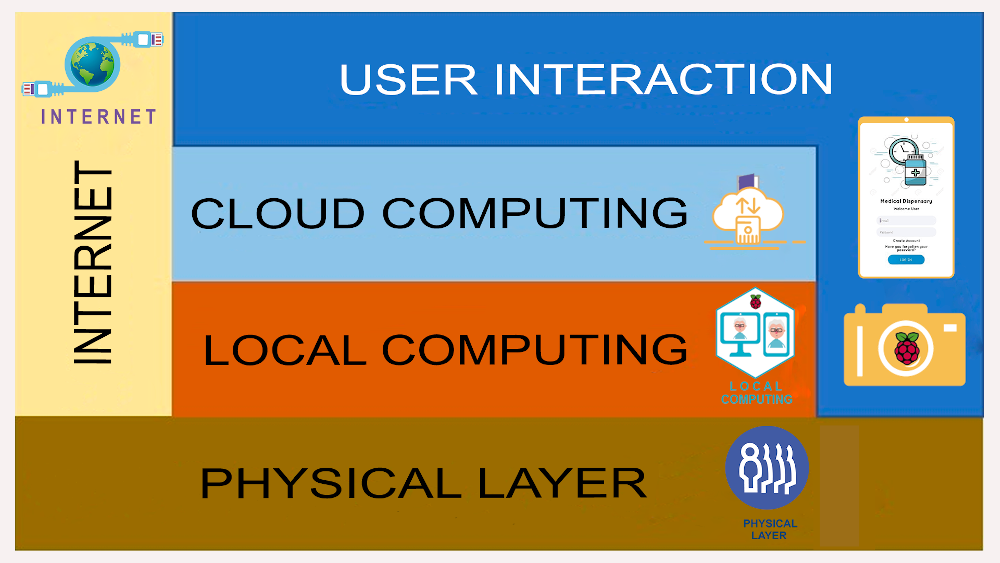
\includegraphics{Architecture.png}
	\caption{Proposed system architecture.}
	\label{figures:architecture}
\end{figure}

\paragraph{Physical Layer. }
It is made up of the sensors and actuators that are embedded into the dispenser (more details and photos about it will be provided in the following subsection). As for sensors, it includes an HC-SR501 passive infrared (PIR) sensor and a Raspberry Pi Camera Board v1.3. The former detects close movements and activates the camera used for facial identification, which is located inside a small slot in the central-front-top part of the dispenser. In addition, it integrates four (Tower Pro Micro Servo 9g SG90) servomotors, which are the actuators that push the corresponding medicine box through one of the four compartments that the dispenser has. These servomotors are controlled by an Arduino Uno R3 microcontroller board. Moreover, the dispenser has an LCD screen, a buzzer and 4 LED lights (one for each of its compartments). Every time a medicine box is dispensed, the LED in that compartment lights up and the buzzer emits a sound to alert the user, while the time and the name of the medicines dispensed are displayed in the LCD screen.

\paragraph{Local Computing. }

This layer registers patients by detecting their faces and taking the necessary photographs to automatically identify them later on. To do so, a mobile app detects people’s faces using the Vision library in AndroidStudio and sends them to a Raspberry Pi 3 model B+. This computing board performs the patient identification through a Python  (version 2.7) application running the OpenCV library (version 2.7). To ensure the privacy of the patient, all his/her personal data that is required by this layer needs either an explicit approval from the own patient or being input under the responsibility of his/her caregiver. Moreover, after the dispenser finalizes a face recognition, it removes all live captured photographs to further avoid any privacy issues.

\paragraph{Cloud Computing. }
We use RESTful cloud services for processing, storage and database management (specifically in PostgreSQL, version 10.8). In addition to storing information in the PostgreSQL database, a folder is created for each patient in which we store the photographs that are used for his/her later identification.

\paragraph{User Interaction. }
The dispenser works non-intrusively. Thus, when the PIR sensor detects any movement near the dispenser, the camera is activated to try to identify if the approaching person is a registered patient. In that case, after identifying him/her, if it is time to take some of his/her medicines, they will be dispensed; otherwise, the time of his/her next dose will be shown on the LCD screen. Another way of interacting with the system would be through the mobile app, which will be used mainly by caregivers. Thus, they will be the ones who will enter the system configuration data, as well as their own data and those of the patients in their care, in addition to their doses of medications and the hours in which they must be taken. The mobile app also serves for the caregiver to receive notifications about whether or not the patient has obtained the medications from the dispenser. If the patient is able to use a smartphone, then he/she could also receive reminders about his/her medicine intakes through the mobile app \cite{r7,r19}. Figure \ref{figures:AppMovil} shows some screenshots of the mobile app. The one on the left (A) shows the menu for the caregiver profile. In it, the \textit{Patients} option gives access to the list of patients who are in charge of the caregiver, as shown in the central capture (B), which also allows adding more patients; the \textit{Dispensers} option would show the list of nearby dispensers, being necessary to have the Bluetooth of the smartphone activated so that it can recognize them; and the \textit{Medicine Boxes} option displays the screenshot (C), which shows bottom-lined buttons to manually dispense the medicine boxes from any of the (four) compartments. This option can be used whenever the patient has not approached the dispenser when he/she should.

\begin{figure}[htb]
	\centering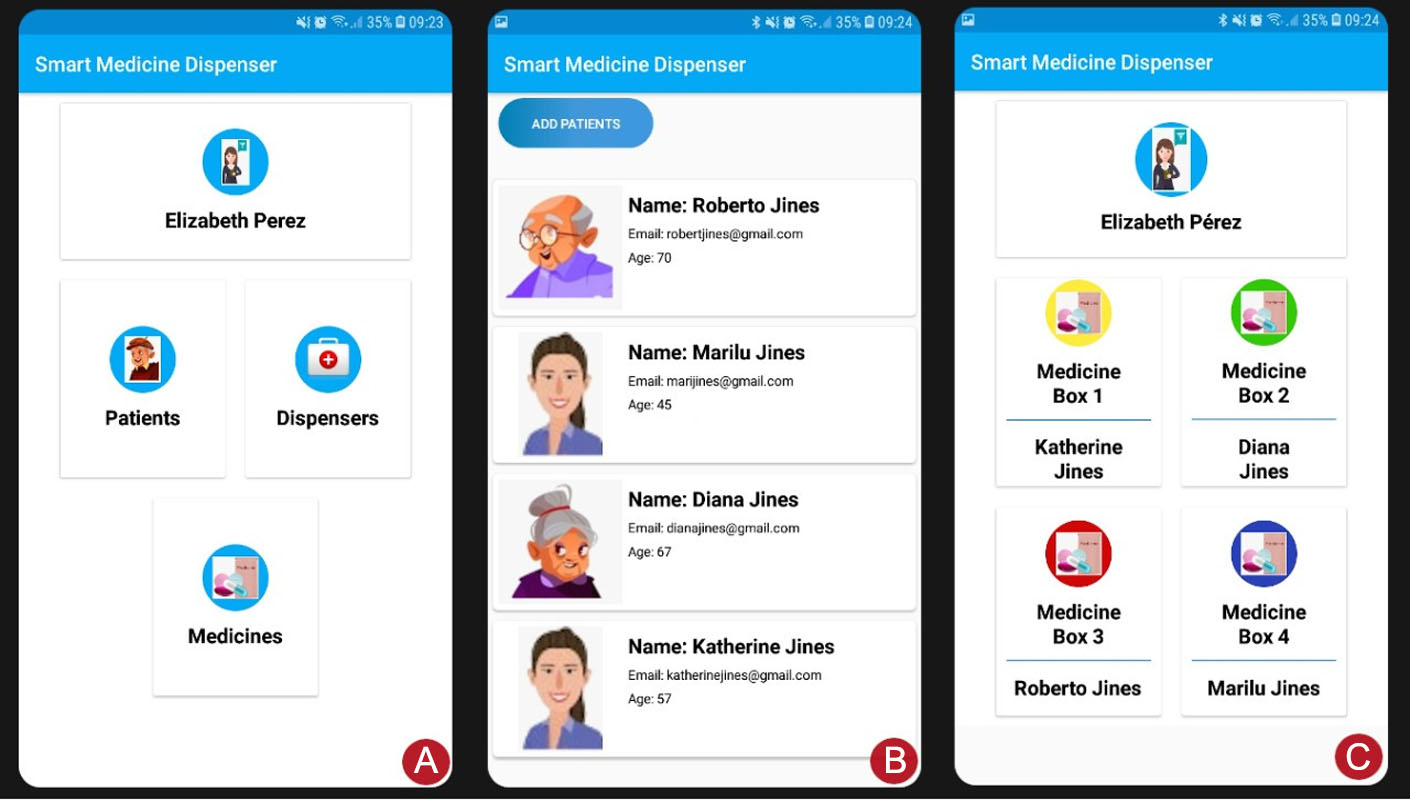
\includegraphics[width=0.93\textwidth]{AppMovilDispenser.png}
	\caption{Some screenshots of the mobile application.}
	\label{figures:AppMovil}
\end{figure}

\paragraph{Internet. }

This layer is essential for IoT-based systems. In our case, the Internet is used for cloud storage of all information and for remote processing when local devices do not have enough resources. All notifications intended for users are issued from a remote system, being also essential to use the Internet for this.

\subsection{Design and Implementation Details}

The design of our smart medicine dispenser is shown in Figure \ref{figures:Diagram}. In it, we can see the different hardware components that make up of the dispenser. It can be powered either by batteries or connected directly to an electrical supply socket.

\begin{figure}[htb]
	\centering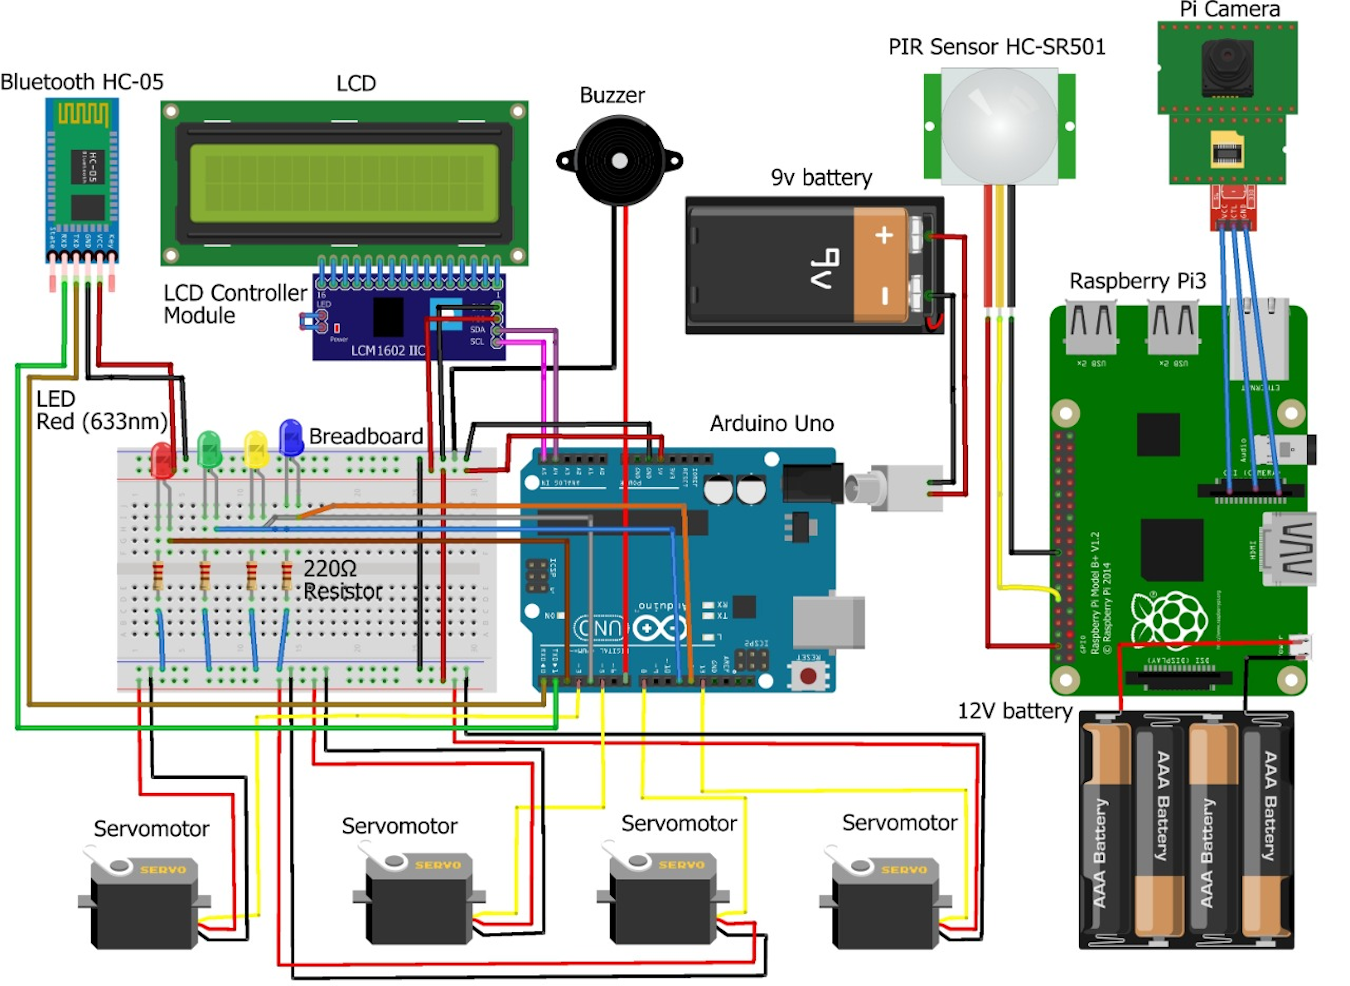
\includegraphics{DispenserDiagram.png}
	\caption{{Design of the smart medicine dispenser showing its hardware components and connections.}}
	\label{figures:Diagram}
\end{figure}

The dispenser is developed to supply the solid medications (pills, capsules,...) that each patient needs to take on schedule. The physical model implemented for the dispenser is shown through several photos in Figure \ref{figures:Dispenser}. The first one (A) shows the internals of the dispenser (with the back cover removed), where we can see two shelves. At the bottom one, there are four servomotors, which are in charge of activating a mechanism with a small rectangular piece that will push the medicine box at the bottom of the corresponding compartment towards the dispenser tray. At the top shelf, we can see the processing components, i.e., an Arduino Uno R3 and a Raspberry Pi 3 model B+, as well as their wiring. The Arduino board controls the servomotors, the Bluetooth module and the LCD screen so that each of these elements fulfils their function, while the Raspberry one manages the facial identification using the camera, as well as the notifications through the LED lights and the sounds emitted by the buzzer. As shown in the top view (B) and in the front view (C) of the dispenser, it has four vertical compartments. In each of them, we can place up to 12 small boxes (48 in total) like the one shown in the fourth photo (D). All the medicines that a patient must take at a certain time should be introduced in one of these boxes. Each box (whose dimensions are 2.5 cm $\times$ 2 cm $\times$ 1 cm) may have a different colour. Normally, the caregiver will fill each box with the corresponding medicines, and will put the boxes inside the dispenser compartments. Note that the dispenser could potentially be shared by 4 patients by assigning a different compartment to each patient.

\begin{figure}[htb]
	\centering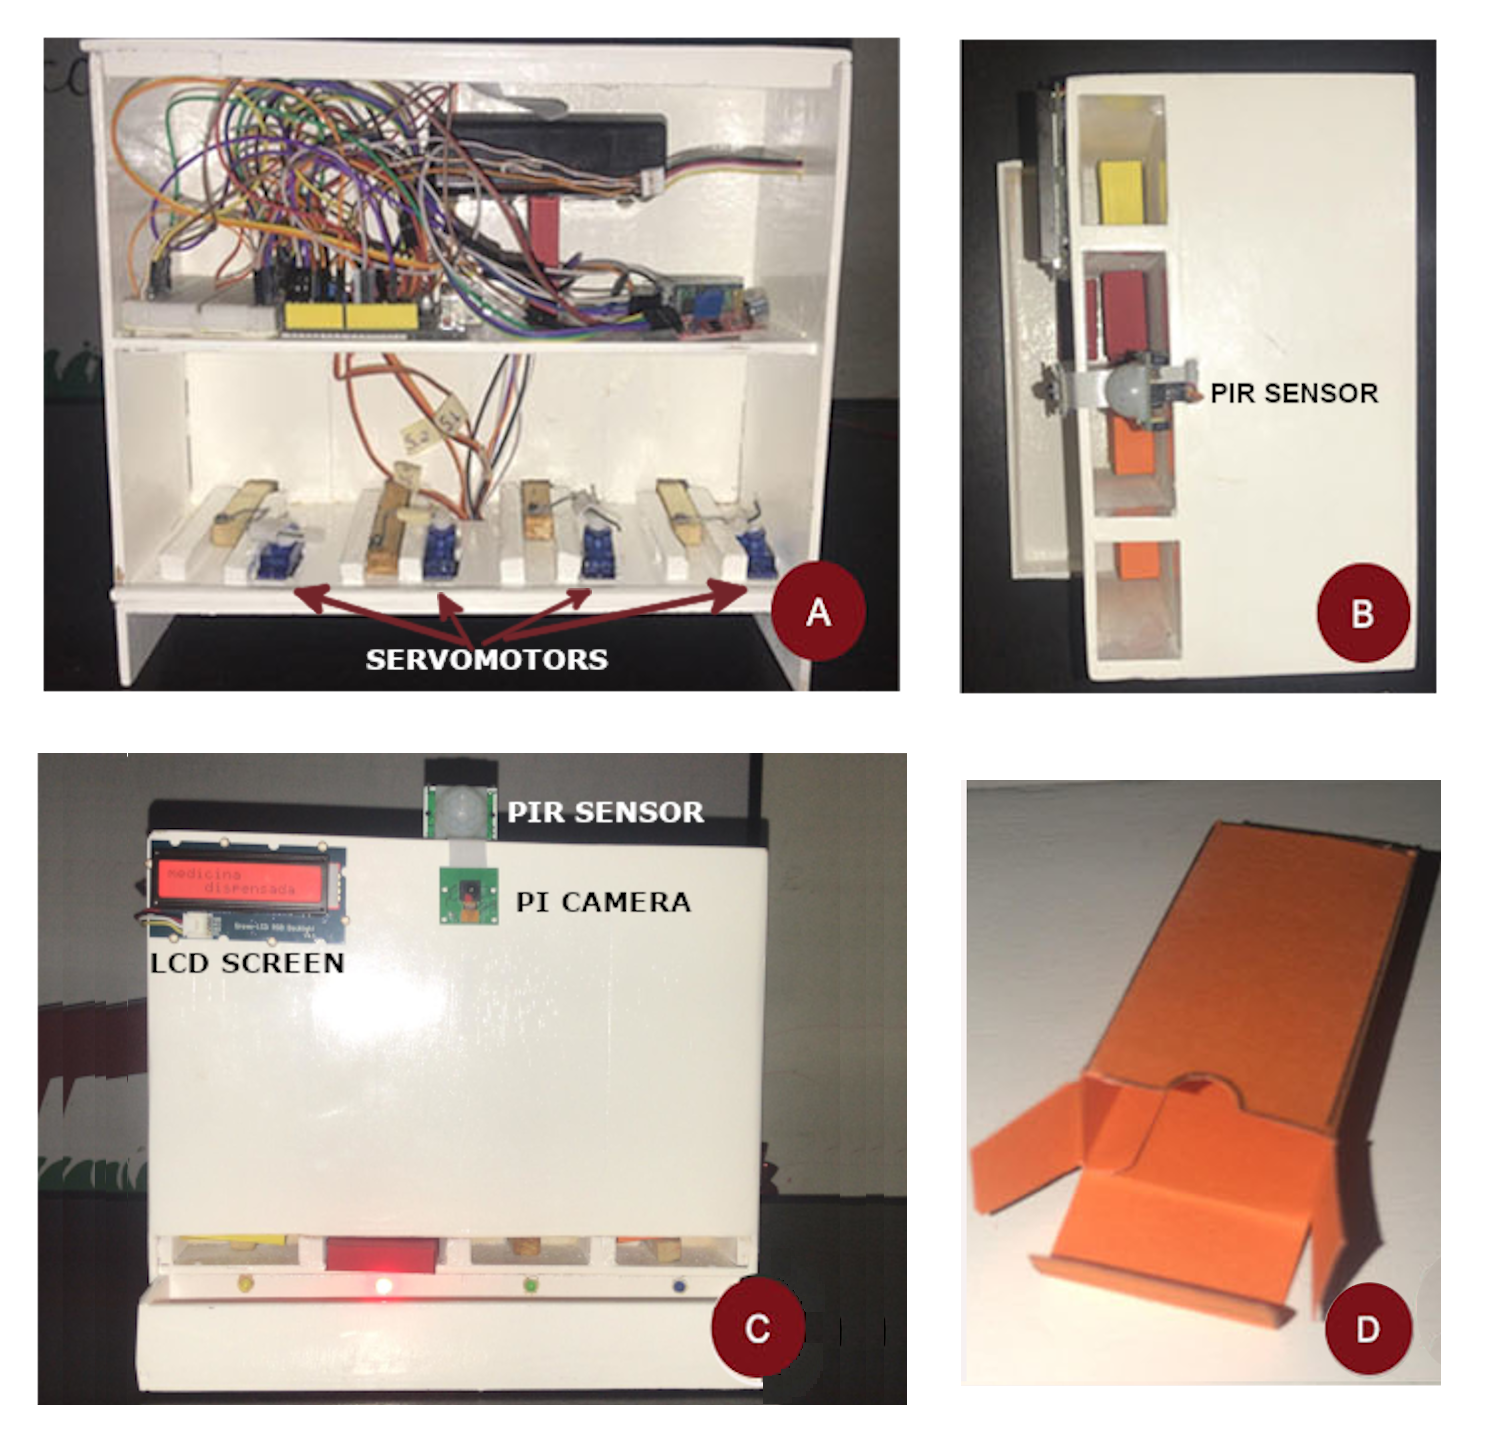
\includegraphics{DispenserViewFinal.png}
	\caption{Photos of both the smart medicine dispenser from different perspectives and one of its medicine boxes.}
	\label{figures:Dispenser}
\end{figure}
\section{Conclusions and Future Work}

We have presented a smart medicine dispenser that helps older people or people with a cognitive problem to take their medicine doses on schedule. In addition, it allows caregivers to supervise that their dependents take their medications on time. Using a facial identification mechanism, it recognizes the patients registered in the system and supplies them with the medicines they should take just when needed. Every time the dispenser provides a medicine box, it generates a sound and illuminates the corresponding compartment. The system also sends remote notifications to caregivers, informing them of the medicines dispensed to their dependents directly on their smartphone. Thus, they can supervise the correct administration of medications and act when necessary (e.g., when somebody forgets to take a dose). In addition, those patients who can use the mobile app may be notified each time they have to take a dose, so that they approach the dispenser to withdraw it.

As for future work, we want to improve the proposed system, closing the dispenser compartments so that they only open when the camera detects the face of the caregiver who must place the medicine boxes in them. This would make it safer. It would also be good for the system to automatically detect which medicines and how many of them the caregiver has put in the different compartments; currently, he/she is who must provide these data through the mobile app. Moreover, an interesting extension would be the automatic request of the necessary medicines to a pharmacy by the system before the patient runs out his/her stock, since this will prevent him/her from losing any intake due to not having a certain medicine. Furthermore, the dispenser could also be integrated into a more general IoT-based system to help elderly people or people with cognitive problems in their daily life.

Besides, the overall system performance will be evaluated after encrypting the whole patient database and face detection images inside the Raspberry Pi, so as to improve patient privacy. Finally, it is important to highlight that our system is currently in use by one real patient, whose feedback will be valuable to develop a refined prototype. That improved prototype will be replicated and delivered to several patients, with different profiles, so as to adequately evaluate the system.

\begin{thebibliography}{99}
\bibitem{r1}
UN Department of Economics and Social Affairs. World Population Prospects - Population Division - United Nations. The International Journal of Logistics Management. Available from: https://population.un.org/wpp/Download/Standard/CSV/.
\bibitem{r2}
Eurostat. Statistics | Eurostat. Life expectancy at birth by sex. 2020. Available from: https://ec.europa.eu/eurostat/databrowser/view/tps00208/default/table?lang=en.
\bibitem{r3}
Baranidharan B. Internet of Things (IoT) Technologies, Architecture, Protocols, Security, and Applications: A Survey. In: Raj P, Raman A, editors. Handbook of Research on Cloud and Fog Computing Infrastructures for Data Science. IGI Global; 2018. India: IGI Global. p. 149–74.
\bibitem{r5}
Guerrero-Ulloa G, Rodríguez-Domínguez C, Hornos MJ. IoT-Based System to Help Care for Dependent Elderly. In: Botto-Tobar M, Pizarro G, Zúñiga-Prieto M, D’Armas M, Zúñiga Sánchez M., editors. Communications in Computer and Information Science. Springer, Cham; 2019. p. 41–55.
\bibitem{r6}
Erazo O, Guerrero-Ulloa G, Guzmán D, Cáceres C. From a Common Chair to a Device that Issues Reminders to Seniors. In: Botto-Tobar M, Zambrano Vizuete M, Torres-Carrión P, Montes León S, Pizarro Vásquez G, Durakovic B, editors. Communications in Computer and Information Science. Quito: Springer; 2020. p. 439–48.
\bibitem{r7}
Singh U, Sharad A, Kumar P. IoMT Based Pill Dispensing System. In: 2019 10th International Conference on Computing, Communication and Networking Technologies, ICCCNT 2019; 2019 jul 6-8; Kampur, India, India. IEEE. p. 1–5. 
\bibitem{r8}
Huang R, Zhao X, Ma J. The Contours of a Human Individual Model Based Empathetic U-Pillbox System for Humanistic Geriatric Healthcare. Future Generation Computer Systems. 2014; 37(July):404–16.
\bibitem{r9}
Jaipriya S, Aishwarya R, Akash NB, Jeyadevi AP. An intelligent medical box remotely controlled by doctor. In: Proceedings of the International Conference on Intelligent Sustainable Systems, ICISS 2019. 2019 Feb 21-22; Palladam, Tamilnadu, India, India. IEEE. p. 565–9.
\bibitem{r10}
Schreier G, Schwarz M, Modre-Osprian R, Kastner P, Scherr D, Fruhwald F. Design and Evaluation of a Multimodal mHealth Based Medication Management System for Patient Self Administration. In: Proceedings of the Annual International Conference of the IEEE Engineering in Medicine and Biology Society, EMBS. 2013 Jul 3-7; Osaka, Japan. IEEE. p. 7270–3.
\bibitem{r11}
Atzori L, Iera A, Morabito G. The Internet Of Things: A Survey. Computer Networks. 2010 Oct 28; 54(15):2787–805.
\bibitem{r12}
Salkin C, Oner M, Ustundag A, Cevikcan E. A Conceptual Framework for Industry 4.0. In: Ustundag A, Cevikcan E, editors. Industry 4.0: Managing The Digital Transformation. Springer, Cham; 2018. p. 3–23.
\bibitem{r13}
Xu H, Yu W, Griffith D, Golmie N. A Survey On Industrial Internet Of Things: A Cyber-Physical Systems Perspective. IEEE Access. 2018 Dec 4; 6: 78238–59.
\bibitem{r14}
Erazo, O, Guerrero Ulloa, G, Santana Sornoza, R, Chávez Boza, B. A Ubiquitous Photo Frame to Provide Reminders to Older Adults. Revista Conrado. 16(72): 34-8.
\bibitem{r15}
Nijiya Jabin Najeeb PK, Rimna A, Safa KP, Silvana M, Adarsh TK. Pill Care-the Smart Pill Box with Remind, Authenticate and Confirmation Function. In: 2018 International Conference on Emerging Trends and Innovations In Engineering And Technological Research, ICETIETR 2018. 2018 Jul 11-13; Ernakulam, India. p. 1–5.
\bibitem{r16}
Kumar SB, Goh WW, Balakrishnan S. Smart Medicine Reminder Device For The Elderly. In: Proceedings - 2018 4th International Conference on Advances in Computing, Communication and Automation, ICACCA 2018. 2018 Oct 26-28; Subang Jaya, Malaysia, Malaysia. IEEE. p. 1–6.
\bibitem{r17}
Jabeena A, Kumar S. Smart medicine dispenser. In: Proceedings of the International Conference on Smart Systems and Inventive Technology, ICSSIT 2018. 2018 Dec 13-14; Tirunelveli, India, India.IEEE. p. 410–4.
\bibitem{r18}
Rumi RI, Pavel MI, Islam E, Shakir MB, Hossain MA. IoT Enabled Prescription Reading Smart Medicine Dispenser Implementing Maximally Stable Extremal Regions and OCR. In: 2019 Third International conference on I-SMAC (IoT in Social, Mobile, Analytics and Cloud) (I-SMAC). 2019 Dec 12-14; Palladam, India, India. IEEE. p. 134–8.
\bibitem{r19}
Kartheek K, Saddam Hussain SK. Medical Dispense System Using IoT. In: Proceedings - International Conference on Vision Towards Emerging Trends in Communication and Networking, ViTECoN 2019. 2019 Mar 30-31; Vellore, India, India. IEEE. p. 1–3. 
\bibitem{r20}
Aneke J, Ardito C, Caivano D, Colizzi L, Costabile MF, Verardi L. A Low-cost Flexible IoT System Supporting Elderly’s Healthcare in Rural Villages. In: ACM International Conference Proceeding Series, AfriCHI '18: 2nd African Conference for Human Computer Interaction. 2018 Dec; Windhoek Namibia. Association for Computing Machinery; p. 184–7.
\bibitem{r21}
Pandey PS, Raghuwanshi SK, Tomar GS. The Real Time Hardware of Smart Medicine Dispenser to Reduce the Adverse Drugs Reactions. In: Proceedings on 2018 International Conference on Advances in Computing and Communication Engineering, ICACCE 2018. 2018 Jun 22-23; Paris, France. IEEE. p. 413–8.
\bibitem{r22}
Arora K, Singh SK. IoT Based Portable Medical Kit. International Journal of Engineering and Advanced Technology. 2019; 8(5 Special Issue 3):42–6.
\bibitem{r4}
Guerrero-Ulloa G, Hornos MJ, Rodríguez-Domínguez C. TDDM4IoTS: A Test-Driven Development Methodology for Internet of Things (IoT)-Based Systems. In: Botto-Tobar M, Zambrano Vizuete M, Torres-Carrión P, Montes León S, Pizarro Vásquez G, Durakovic B, editors. Communications in Computer and Information Science. Quito: Springer; 2020. p. 41–55.
\bibitem{r23}
Hornos MJ. Application of Software Engineering Techniques to Improve the Reliability of Intelligent Environments. Journal of Reliable Intelligent Environments. 2017; 3(1):1-3.
\bibitem{r24}
Hornos MJ, Rodríguez-Domínguez C. Increasing User Confidence in Intelligent Environments. Journal of Reliable Intelligent Environments. 2018; 4(2): 71-3.
\end{thebibliography}

\end{document}
